%!TEX root = ../ap_gcc.tex

\section{CMake Build System} CMake is a great tool for managing complex cross platform build processes. The general idea is not to create just another build system, but to automatically generate configuration or project files for widely used build systems and IDEs.

To build a project using CMake, \pathname{CMakeLists.txt} files need to get created. Those files contain information on files to build, paths to include, libraries and executables to create, pre and post build activities and much more.

There are no special things to consider while writing code which will be build using CMake.

The \toolname{cmake} command line utility uses the \pathname{CMakeLists.txt} files to generate for example Visual Studio project files or Makefiles.

\subsection{Finding Dependencies} One of CMake's great features is to automatically find libraries the code depends on. This is done by special scripts. Usually, those scripts search in common paths like \pathname{/usr/include} and \pathname{/usr/lib} for certain patterns like a library file name or a header file. Hence, this feature is very useful on Unix platforms. On Windows, it is common to set dependency paths in the CMake GUI. See below for details.

We added a script for finding VRS. If VRS is not installed but located in some custom path, or you are using a Windows platform, the variable \inlinecode{VRS\_DIR} can be set to the VRS root directory. See below how this is done.

\subsection{On Mac OS X} When we built CGA on Mac OS X, we always used Makefiles. It should be no problem to generate XCode project files, but this is how it is done using Makefiles.

We create a new directory for CMake generated files. This keeps the project structure clean.
\begin{verbatim}
$ cd path/to/cga/root
$ mkdir build
$ cd build
$ VRS_DIR="/my/path/to/vrs/" cmake -G "Unix Makefiles" ..
$ make
\end{verbatim}

After make is done, all the build results are placed in the \pathname{build} directory. For example, the CGA application can be executed like this:
\begin{verbatim}
$ open cga/cgaapplication/cga.app
\end{verbatim}

\subsection{On Linux} Since we are using Makefiles on Linux and Mac OS X, the process on both platforms is the same. So please, refer to the Mac OS X section to see how to build CGA on Linux using CMake.

After the build process is done, the CGA Application can be executed like this:
\begin{verbatim}
$ ./cga/cgaapplication/cga
\end{verbatim}

By the way, on Linux there is, like on Windows systems, a GUI that helps configuring a CMake project.

\begin{figure}[ht]
\centering
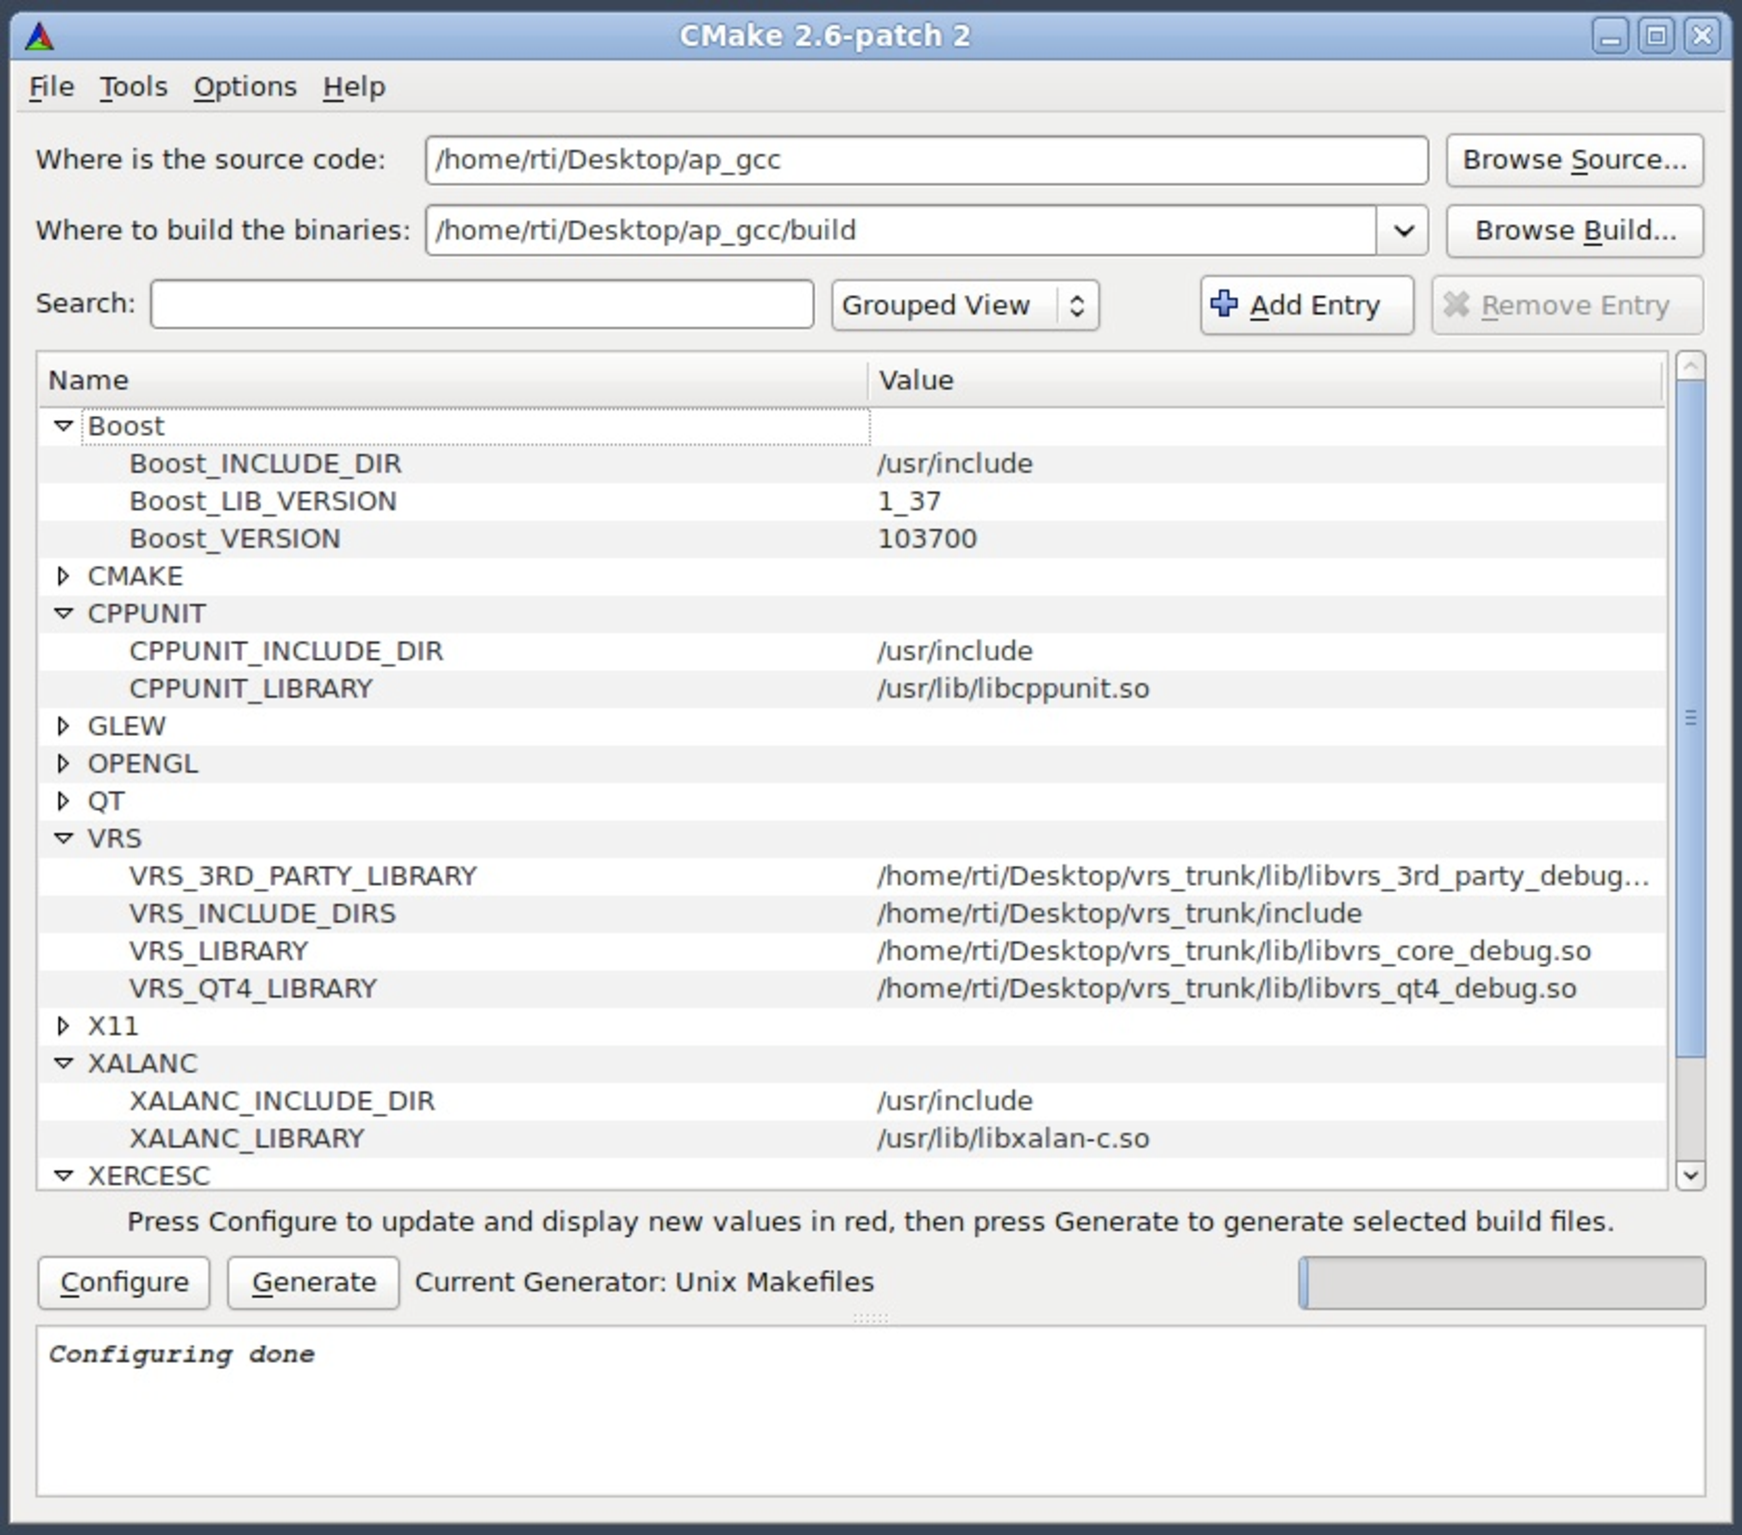
\includegraphics[width=10cm]{images/cmake_gui_linux}
\caption{CMake GTK GUI on Ubuntu Debian Linux}\label{fig:cmake_gui_linux}
\end{figure}


\subsection{On Windows}
Since on Windows the automatic dependency finding does not work like on unix systems (because it is not possible to predict where libraries and headers of dependencies are placed) some more steps are needed, but all of them are straight forward. You need the CGA dependency package on your system.

\begin{itemize}
	\item Start up the CMake GUI
	\item Set the source code directory to the CGA root directory
    \item Set the build directory to a newly created directory inside the CGA root directory (you might want to call it \pathname{build})
    \item Hit the configure button (lots of red lines should appear in the GUI)
    \item Point all the red marked paths to the correct locations of dependency headers and libraries
    \item Hit the configure button again, all red lines should disappear now
    \item Hit the generate button
    \item Inside the \pathname{build} folder a new file named \pathname{cga.sln} was created
    \item Open this file with Visual Studio
    \item Build the solution
\end{itemize}


\todo{CMake GUI screenshot}

\subsection{Qt specific build steps} Building projects using Qt requires additional build steps like running \toolname{uic} and \toolname{moc}. CMake provides special commands for that: \inlinecode{QT4\_WRAP\_UI}, \inlinecode{QT4\_WRAP\_CPP} and \inlinecode{QT4\_ADD\_RESOURCES}. Generated files are placed in \pathname{build/cga}.
